\documentclass[conference]{IEEEtran}
\usepackage[T1]{fontenc}
\usepackage{amsmath,booktabs,graphicx,array}
\usepackage[hidelinks]{hyperref}
\usepackage{url}
\begin{document}
\title{Outcome Language and Appellate Classification:\\MVP and Evaluation Pipeline Checkpoint}
\author{\IEEEauthorblockN{Hyun Sang Ryu, Becca Weng, and Yinkui Yu}
\IEEEauthorblockA{Team 11, CS-GY 6923-INET Machine Learning\\New York University\\October 25, 2026}}
\maketitle

\begin{abstract}
We have built an end-to-end system for classifying published New York private-property slip/trip-and-fall appeals as affirmed or reversed/vacated. The current team-reviewed pool contains 120 candidates: 86 training cases, 16 validation cases, 17 reserved test cases, and one case held for an unresolved companion appeal. The system combines versioned preprocessing, case-family splits, a majority baseline, TF-IDF logistic regression and linear SVM, and frozen LEGAL-BERT features with logistic regression. We compare complete cleaned opinions with text that removes direct outcome statements, and include five matched-length random-removal controls. At fixed regularization, validation balanced accuracy changes from 0.688 to 0.625 for logistic regression, 0.750 to 0.500 for SVM, and 0.875 to 0.5625 for LEGAL-BERT after masking. Random-removal logistic regression averages 0.675. These preliminary findings show that the pipeline is operational and suggest sensitivity to outcome language, but the small validation set and collateral removal of useful reasoning limit interpretation. The final test period has not been evaluated.
\end{abstract}
\begin{IEEEkeywords}
legal text classification, outcome masking, LEGAL-BERT, evaluation pipeline, MVP
\end{IEEEkeywords}

\section{Working Core System / MVP}
Our research question is: \emph{How well can classifiers identify appellate outcomes after direct outcome statements are removed, and do frozen legal-language representations help compared with TF-IDF?} Opinions are written after a ruling, so our task is classification of published decisions, not prediction of future judgments. This distinction follows the concerns about task and data alignment discussed by Medvedeva and McBride~\cite{medvedeva}.

The core system is now working from saved source opinions through predictions and evaluation. It validates input files, joins reviewed targets by case ID, preserves case-family assignments, prepares FULL/MASKED inputs, fits baselines and classifiers, and produces metrics, figures and case-level error records. The accompanying notebook executes these steps with explanations and comments. Its final check independently recomputes 34 model/regularization-condition results on the same 16 validation cases.

This checkpoint builds on Becca's merged preparation PRs~12--15 and Hayden's six accepted additions in PR~16. We integrated them in a new dataset version while retaining the original submissions and earlier trial. The team confirmed independent review of their work on October~25; the new dataset is marked \emph{team-reviewed}. The old provisional trial is a separate historical result. Our record does not establish an additional blinded annotation study or new inter-human agreement measurement.

The work is deliberately manageable. LEGAL-BERT supplies frozen features rather than a fine-tuned model, following the representation motivation of Chalkidis et al.~\cite{legalbert}. LLM-assisted annotation helped organize the original records, but acceptance is recorded separately from those drafts. Prior work on LLM-generated training labels~\cite{llmlabels} motivates assistance, not treating generated evidence quotations as sufficient validation.

\section{Data and Evaluation Pipeline}
\subsection{Scope, Labels and Current Coverage}
The saved CourtListener retrieval contains 4,232 candidate opinion clusters from New York's Appellate Division, 2010--2024. Initial screening retained 506 provisional cases. For this MVP we use Partition~A's 169 candidates, rather than presenting all 506 as reviewed modeling examples.

Eligibility concerns an injured person's negligence claim after a slip/trip and fall on supported private property. Procedural-only appeals, unrelated claims, unclear property status, and mixed/unclear appellate outcomes remain outside the binary task. Label~0 means the appealed order/judgment is affirmed in full; label~1 means reversed or vacated in full. ``Insofar as appealed from'' can qualify when the entire current appeal has one outcome. These labels do not identify the winning party: a reversal can favor a defendant.

All three original annotation submissions marked 114 cases include and agreed on their binary labels. Hayden accepted six more candidates, giving 120 selected cases. The remaining 35 review cases and 14 cases withheld under the team's selection rule are not used. Sodhi remains in the selected pool but outside modeling while its companion appeal is unresolved. Thus, 119 cases are assigned, and 102 training/validation cases enter this run. The selected pool remains below the proposal's 150-reviewed-case MVP target; we report the actual coverage rather than relax eligibility to meet a number.

\begin{table}[t]
\caption{Fixed chronological assignments after the six additions.}
\label{tab:splits}
\centering\footnotesize
\begin{tabular}{llrrr}
\toprule Period & Use & Affirmed & Reversed & Total \\
\midrule
2010--2020 & Training & 59 & 27 & 86 \\
2021--2022 & Validation & 8 & 8 & 16 \\
2023--2024 & Reserved test & 12 & 5 & 17 \\
\midrule
Unassigned & Family hold & 1 & 0 & 1 \\
\bottomrule
\end{tabular}
\end{table}

Before team acceptance, pairwise eligibility agreement among the original LLM-assisted submissions ranged from 86.4\% to 92.3\% over 169 cases; Cohen's $\kappa$ ranged from 0.670 to 0.824. These are draft-agreement diagnostics, not agreement with an independent human-gold sample. They also show why unanimous agreement on binary outcomes alone does not settle eligibility.

\subsection{Splits, Families and Feature Boundaries}
We retain the proposal's chronological boundaries (Table~\ref{tab:splits}) and all of Becca's existing assignments. Five additions fall in training and one in the reserved test period. Her saved family screen covers all 506 opinions, with 495 observed families. Selected records have no known family crossing a split. Calibration exposure propagates across linked publication variants and is restricted to training. Family screening is not proof that every possible relationship has been found.

Only opinion text enters vectorization/tokenization. Labels, identifiers, extracted findings, selected evidence quotations and review notes are kept in separate target or audit fields. Vocabulary, inverse-document frequencies, feature scaling and class weights are fitted on training data only. Every chunk inherits its parent case's split; chunks never become independent evaluation examples.

The integration checks exact IDs, text hashes, shared targets, source versions and family restrictions. An LF-canonical file adapter resolves Windows checkout line endings and a path-separator issue in the supplied loader, while retaining its structural validator and checksum requirements. Existing development FULL/MASKED texts are reproduced exactly. The new training cases use the same frozen preprocessing functions without case-specific overrides.

\subsection{Text Versions and the Masking Audit}
FULL uses Becca's \texttt{full\_v1} cleaning to remove recognized web/publication metadata and separate dissent material while preserving the controlling opinion. MASKED uses her frozen \texttt{masked\_v2} rules to remove disposition blocks and sentences directly stating the current appeal's result. The same rules apply to both classes; labels and annotation evidence are not masking inputs. We preserve removed passages with offsets, reason codes and word-loss counts.

To address the first feedback point, we performed an additional pre-model audit of two cases per class in both training and validation, eight in total. The coding assistant read each full cleaned opinion and removed passage. All sampled whole-appeal dispositions were removed while substantial reasoning and earlier-decision references remained. For example, v2 retains the historical ruling in \emph{Cheprakova} and an evidentiary ruling in \emph{Yerry} that the previous trial mask removed unnecessarily. These findings did not trigger validation-specific rule changes.

The audit also records limits. Some removed sentences combine direct outcomes with reasoning or citations. An ancillary leave-to-appeal ruling remains in \emph{Zubillaga}. A small sample cannot establish exhaustive cue removal. Across the 102 development cases, masking removes an average 9.67\% of words per opinion, with median 8.13\% and maximum 57.05\%; the largest loss is in a very short opinion. Table~\ref{tab:length} distinguishes word and tokenizer lengths.
\begin{table*}[t]
\caption{Development text lengths. Tokens exclude CLS/SEP and padding; one model input holds 510 content tokens.}
\label{tab:length}
\centering\scriptsize
\begin{tabular}{llrrrrrrrrrrrr}
\toprule & & \multicolumn{5}{c}{Words} & \multicolumn{5}{c}{Content tokens} & $>510$ & Total \\
\cmidrule(lr){3-7}\cmidrule(lr){8-12}
Split & Text & Min & Median & Mean & P90 & Max & Min & Median & Mean & P90 & Max & tokens & chunks \\
\midrule
Train & FULL & 149.0 & 467.5 & 511.0 & 831.5 & 1486.0 & 213.0 & 638.5 & 700.9 & 1169.5 & 1878.0 & 66.3\% & 156 \\
Train & MASKED & 64.0 & 424.0 & 469.7 & 772.5 & 1425.0 & 82.0 & 590.5 & 646.0 & 1098.5 & 1788.0 & 61.6\% & 151 \\
Validation & FULL & 276.0 & 534.0 & 650.9 & 925.5 & 1796.0 & 375.0 & 714.0 & 868.2 & 1252.0 & 2320.0 & 87.5\% & 36 \\
Validation & MASKED & 250.0 & 507.5 & 596.1 & 872.0 & 1671.0 & 331.0 & 679.0 & 796.1 & 1208.0 & 2147.0 & 81.2\% & 34 \\
\bottomrule\end{tabular}
\end{table*}

\section{Baselines and Model Implementation}
\subsection{Majority and Lexical Baselines}
The majority baseline always predicts affirmed, the most frequent training label. Because validation is balanced, it obtains accuracy and balanced accuracy 0.500, but macro F1 only 0.333. TF-IDF logistic regression and linear SVM are our substantive baselines, rather than comparing a language representation only against majority guessing.

Both lexical models use word unigrams/bigrams, \texttt{min\_df=2}, at most 30,000 features and L2-normalized vectors. Logistic regression uses L2 regularization; both classifiers use balanced training-derived class weights. We try $C\in\{0.1,1,10\}$, selecting validation balanced accuracy, then macro F1, then smaller $C$ to break ties. Separately, the main text-intervention comparison fixes $C=1$ in advance to avoid changing text and regularization simultaneously.

\subsection{Frozen LEGAL-BERT Features}
We use \texttt{nlpaueb/legal-bert-base-uncased} with encoder and tokenizer revision \texttt{15b570cbf88259610b082a167dacc190124f60f6}. The checkpoint's slow uncased tokenizer is used without truncation. Each opinion is divided into non-overlapping chunks of at most 510 content tokens, with CLS/SEP added separately. All chunks, including a short last chunk, are retained.

The encoder runs frozen in evaluation/inference mode. We mean-pool final-layer content-token vectors, excluding special tokens and padding. For chunks with $n_j$ content tokens and mean vectors $\mathbf{h}_j$, the opinion vector is
\begin{equation}
\mathbf{h}=\frac{\sum_j n_j\mathbf{h}_j}{\sum_j n_j}.
\end{equation}
This yields one 768-dimensional vector per opinion and text variant. Attention is local to each chunk, so using all tokens does not mean modeling unrestricted cross-chunk context. A training-fitted StandardScaler and balanced logistic regression use the same $C$ grid. We cache features with case IDs, text hashes and the pinned representation settings. The run processed 192 FULL and 185 MASKED chunks across the 102 development opinions.

\section{First Experiments and Evaluation}
Experiment~1 compares the three learned models on FULL and MASKED, giving six primary conditions, plus majority. We report accuracy, balanced accuracy, macro F1, class counts, and raw/row-normalized confusion matrices with true labels as rows and fixed class order $[0,1]$. Balanced accuracy averages the two class recalls; it equals accuracy on this particular balanced validation set. Per-class recall helps explain otherwise similar scores.

Experiment~2 prioritizes the requested random-text-removal control for TF-IDF logistic regression. For each opinion, five fixed seeds (11, 23, 37, 51, 71) shuffle sentence indices and remove text until the MASKED word-loss budget is reached. A random contiguous part of the final selected sentence matches that budget exactly. All sentences, including outcome statements, are eligible; accidental removal of identified outcome words is logged. Every seed is reported. This controls word quantity, not semantic content or subword-token count.

Experiment~3 examines errors, training coefficients and opinion length. We provide all 16 validation cases in the error packet rather than claiming 20 unique examples from this set. Length groups use fixed FULL-word boundaries of 400 and 800, with group and class counts alongside scores.

We also implement 5,000 paired family-bootstrap resamples for descriptive validation intervals. FULL and MASKED use the same sampled families. A replicate missing either class would be skipped and counted; none were skipped here. These intervals are not final-test intervals and do not correct for earlier development reuse or dataset selection. Final-test evaluation and its paired intervals remain deferred until the final pipeline is fixed.

\section{Preliminary Results}
\begin{table}[t]
\caption{Preliminary validation results at fixed $C=1$. All conditions use the same 16 cases (8 per class).}
\label{tab:results}
\centering\footnotesize
\begin{tabular}{llrrr}
\toprule Model & Text & Acc. & Bal. acc. & Macro F1 \\
\midrule
Majority & -- & 0.500 & 0.500 & 0.333 \\
TF-IDF LR & FULL & 0.688 & 0.688 & 0.676 \\
TF-IDF LR & MASKED & 0.625 & 0.625 & 0.600 \\
TF-IDF SVM & FULL & 0.750 & 0.750 & 0.733 \\
TF-IDF SVM & MASKED & 0.500 & 0.500 & 0.418 \\
LEGAL-BERT LR & FULL & 0.875 & 0.875 & 0.875 \\
LEGAL-BERT LR & MASKED & 0.562 & 0.562 & 0.561 \\
\bottomrule\end{tabular}
\end{table}
\begin{table}[t]
\caption{LR random-removal controls at $C=1$. SD describes seed variability, not a confidence interval.}
\label{tab:control}
\centering\footnotesize
\begin{tabular}{lrrr}
\toprule Seed & Acc. & Bal. acc. & Macro F1 \\
\midrule
11 & 0.625 & 0.625 & 0.600 \\
23 & 0.688 & 0.688 & 0.676 \\
37 & 0.750 & 0.750 & 0.746 \\
51 & 0.625 & 0.625 & 0.600 \\
71 & 0.688 & 0.688 & 0.676 \\
\midrule
Mean & 0.675 & 0.675 & 0.660 \\
SD & 0.052 & 0.052 & 0.061 \\
\bottomrule\end{tabular}
\end{table}
\begin{figure*}[t]
\centering
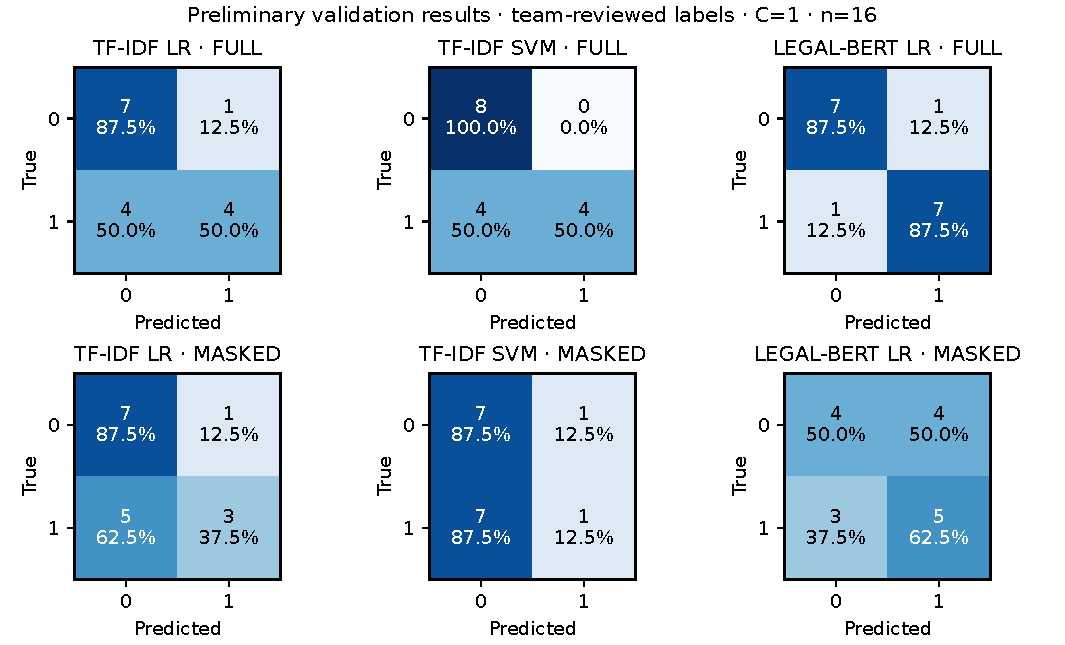
\includegraphics[width=0.94\textwidth]{images/confusion_matrices.pdf}
\caption{Fixed-$C$ validation confusion matrices. Entries show counts and row-normalized percentages. Label 0 is affirmed; label 1 is reversed/vacated. These are preliminary results on team-reviewed data.}
\label{fig:confusion}
\end{figure*}

\subsection{Outcome Language and Text Loss}
Table~\ref{tab:results} shows that masking reduces balanced accuracy for all three models at fixed $C=1$. LR drops by 0.0625, SVM by 0.2500, and LEGAL-BERT by 0.3125. LEGAL-BERT has the highest FULL score, but its MASKED score does not exceed LR's at these fixed settings. We cannot infer a stable ranking from 16 validation cases: one error changes accuracy by 6.25 percentage points.

Random removal gives LR mean balanced accuracy 0.675 with standard deviation 0.052 across seeds (Table~\ref{tab:control}), compared with 0.688 for FULL and 0.625 for MASKED. The pattern is consistent with outcome-directed removal having a larger effect than generic text loss on this sample. It is not a clean causal estimate: masking can remove useful reasoning, while random removal can also remove outcome language. The random-seed variation is substantial relative to the observed difference.

When $C$ is selected on validation, MASKED LR ($C=1$), SVM ($C=0.1$), and LEGAL-BERT LR ($C=10$) all reach balanced accuracy 0.625; their macro F1 values are 0.600, 0.600 and 0.625, respectively. FULL LR selects $C=10$ and reaches 0.750. These are secondary development scores on the selection set, not unbiased estimates. The fixed-$C$ table remains the main controlled comparison.

\subsection{Class Errors and Qualitative Findings}
Figure~\ref{fig:confusion} shows why aggregate accuracy alone is insufficient. After masking, reversal recall is 3/8 for LR, 1/8 for SVM and 5/8 for LEGAL-BERT. LEGAL-BERT's better reversal recall is offset by only 4/8 affirmance recall. A claim that it simply ``understands the law better'' is not supported by these results.

In \emph{Schneider v. Gap}, all three models change from correct on FULL to incorrect on MASKED. The retained reasoning favors the defendant, but the earlier court had denied the defense motion; the appellate defense victory is therefore a reversal. This illustrates the need to connect merits reasoning to the appealed ruling, rather than equate party success with affirmance. In \emph{Zubillaga}, LEGAL-BERT changes from correct to incorrect after masking, while both lexical models are incorrect in both versions. Its long procedural history and multiple orders remain possible sources of confusion even though every chunk is processed.

There are counterexamples to a simple representation story. In \emph{Yerry}, LEGAL-BERT is correct with both texts while the lexical models are wrong. In \emph{Cheprakova}, both lexical models remain correct while LEGAL-BERT becomes incorrect after masking, despite retained causation reasoning. These are possible failure explanations, not direct observations of model reasoning.

Training LR coefficients associate citation-style terms such as ``1st dept'' with affirmed, and terms such as ``parking'' and ``rug'' with reversed. Such associations may reflect writing style or case mix. A department cited in an opinion does not necessarily identify its deciding court, and a coefficient is not a causal explanation.

\begin{table}[t]
\caption{Descriptive validation bootstrap: 95\% intervals for balanced accuracy and paired FULL--MASKED difference at $C=1$.}
\label{tab:bootstrap}
\centering\footnotesize
\setlength{\tabcolsep}{3pt}
\begin{tabular}{lrrr}
\toprule Model & FULL & MASKED & Difference \\
\midrule
TF-IDF LR & [0.46, 0.89] & [0.41, 0.82] & [0.00, 0.20] \\
TF-IDF SVM & [0.57, 0.93] & [0.33, 0.67] & [0.06, 0.47] \\
LEGAL-BERT LR & [0.69, 1.00] & [0.31, 0.81] & [0.02, 0.60] \\
\bottomrule\end{tabular}
\end{table}
The bootstrap intervals in Table~\ref{tab:bootstrap} are wide. Although some paired difference intervals are above zero in this development sample, repeated validation use, small class counts and masking imperfections prevent a strong inferential claim. We will not use these intervals as a reason to stop reviewing data or to open the test set early.

\section{Checkpoint Status and Next Steps}
The checkpoint's five requested components are present: (1) an end-to-end working MVP; (2) a versioned data/evaluation pipeline; (3) majority and credible lexical baselines; (4) completed masking and random-removal experiments; and (5) preliminary quantitative and qualitative evidence. The notebook contains executable stages and verification rather than only loading a results table. Generated LaTeX tables and figures use the same saved metrics.

The main limitations are sample size, selection of published and relatively unambiguous cases, repeated validation use, remaining outcome cues, collateral deletion, possible unobserved family links, and unknown overlap with encoder pretraining data. Team review was confirmed on October~25, but a separate per-case blinded-review protocol was not newly logged in this integration. We therefore describe the data as team-reviewed without claiming a new independent human-gold benchmark. Results from the earlier trial and this run are not a controlled before/after comparison, because both selection and preprocessing changed.

Next we will resolve the remaining eligibility and companion questions, expand reviewed coverage while preserving the natural class distribution, and document the evaluation-review process. We will refine any masking rules using training cases, version the change, and rerun all affected conditions. Once the final pipeline is fixed, we will evaluate the reserved test period once and report paired family-bootstrap uncertainty. We will prioritize this investigation over adding model complexity. No claim of prospective legal prediction is intended.

\section*{Reproducibility and Contributions}
Becca prepared the source cleaning, family/split manifests, MASKED v2 and length pipeline; Hayden supplied domain review and six accepted additions; Yinkui integrated the reviewed version, ran models/evaluation and prepared the notebook/report. The current notebook is \texttt{experiments/mvp\_a/Team\_11\_MVP.ipynb}; artifacts include input hashes, settings, removed spans, predictions, all metrics and the eight-case audit. Upstream data are pinned to main commit \texttt{ecca2a4}; the representation revision is fixed above. Experiment seed is 20261025. No test predictions were generated.

\begin{thebibliography}{3}
\bibitem{medvedeva} M. Medvedeva and P. McBride, ``Legal Judgment Prediction: If You Are Going to Do It, Do It Right,'' in \emph{Proc. Natural Legal Language Processing Workshop}, 2023, pp. 73--84. \url{https://aclanthology.org/2023.nllp-1.9/}
\bibitem{legalbert} I. Chalkidis, M. Fergadiotis, P. Malakasiotis, N. Aletras, and I. Androutsopoulos, ``LEGAL-BERT: The Muppets straight out of Law School,'' in \emph{Findings of EMNLP}, 2020, pp. 2898--2904. \url{https://aclanthology.org/2020.findings-emnlp.261/}
\bibitem{llmlabels} N. Pangakis and S. Wolken, ``Knowledge Distillation in Automated Annotation: Supervised Text Classification with LLM-Generated Training Labels,'' arXiv:2406.17633, 2024. \url{https://arxiv.org/abs/2406.17633}
\end{thebibliography}
\end{document}
